\documentclass[../TDO1-O2.tex]{subfiles}%

\begin{document}
\section[s]"3"{Fibre optique à saut d'indice}

\enonce{%
	Les câbles à fibres optiques permettent la transmission à haut débit de tous
	types de signaux électromagnétiques, sur de longues distances avec très peu
	d'atténuation~; ceux-ci se propagent comme la lumière. Chaque câble comporte un
	grand nombre de fibres très fines.

	Une fibre optique à saut d'indice peut être assimilée à un cylindre de
	révolution d'axe $Oz$, constitué d'un cœur de rayon $a$ (de l'ordre de 8 à
	\SI{50}{\micro m}) et d'indice $n_1$, entouré d'une couche cylindrique appelée
	\textit{gaine}, d'épaisseur $b-a$ et d'indice $n_2 < n_1$.

	\begin{figure}[h]
		\centering
		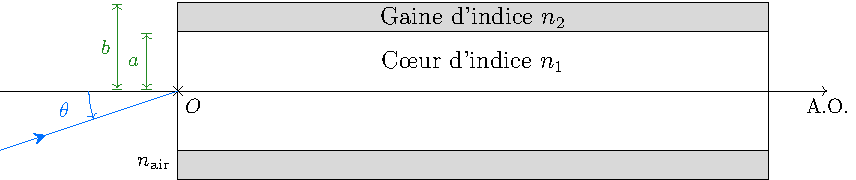
\includegraphics[width=.8\linewidth]{fibre_plain.pdf}
		\captionsetup{justification=centering}
		\caption{Schéma d'une fibre optique à saut d'indice.}
		\label{fig:fibre_plain}
	\end{figure}

	Un rayon pénètre depuis l'air dans la fibre par sa base en $O$, en faisant un
	angle $\theta$ avec l'axe optique confondu avec $Oz$.
}%

\QR{%
	Exprimer une condition sur $\theta$ en fonction des indices $n_1$ et
	$n_2$ pour que le rayon ne se propage uniquement dans le cœur de la fibre.
}{%
	\begin{figure}[h]
		\centering
		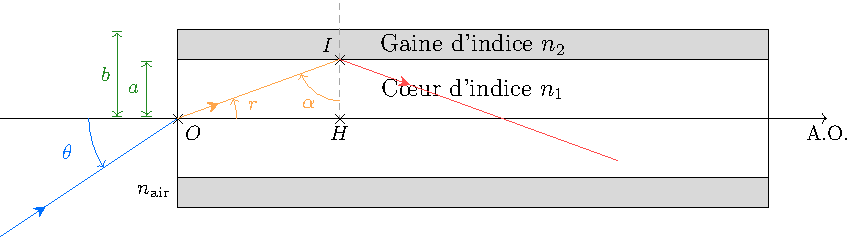
\includegraphics[width=.8\linewidth]{fibre.pdf}
		\captionsetup{justification=centering}
		\caption{Schéma d'une fibre optique à saut d'indice.}
		\label{fig:fibre}
	\end{figure}
	\begin{tcolorbox}[blankest]
		\begin{isd}
			\begin{itemize}
				\olditem[En O] : $\sin(\theta) = n_1\sin(r) \Leftrightarrow \fbox{$\DS\sin(r) =
							\frac{\sin(\theta)}{n_1}$}$~;
				\olditem[OIH] : $\alpha = \DS \frac{\pi}{2} - r$~;
				\olditem[En I] : On veut $\sin(\alpha) \geq \DS\frac{n_2}{n_1}$~;
				\olditem[$\alpha\rightarrow r$] : $\sin(\alpha) = \sin(\pi/2 -r) =
					\cos(r)$\\
				\fbox{$\DS\sin(\alpha) \geq \frac{n_2}{n_1} \Leftrightarrow \cos(r) \geq
						\frac{n_2}{n_1}$}
			\end{itemize}
			\tcblower
			\begin{itemize}[leftmargin=100pt]
				\olditem[$\cos(r)\rightarrow\sin(r)$] : $\cos^2(r) = 1-\sin^2(r)$~;
				\olditem[$r\rightarrow\theta$] : $\sin^2(r) = \DS
					\frac{\sin^2(\theta)}{n_1{}^2}$~;
				\olditem[Combinaison] : $n_1{}^2 - \sin^2(\theta) \geq n_2{}^2$~;
				\olditem[Conclusion] : \fbox{$\theta \leq \arcsin \left( \sqrt{n_1{}^2 -
							n_2{}^2} \right)$}
			\end{itemize}
			C'est ce qu'on appelle le \textbf{cône d'acceptance}.
		\end{isd}
	\end{tcolorbox}
}%

\QR{%
Déterminer l'écart temporel entre la sortie du rayon le plus rapide
(en ligne droite) et le rayon le plus lent ($\th = \th_{\lim}$).
}{%
Soit $L$ la longueur de la fibre optique. Un rayon entre dans la fibre
avec un angle d'incidence $\th$ variable, compris entre 0 et $\th_{\lim}$.
\smallbreak
Le rayon le plus rapide parcourt la distance $L$ à la vitesse $c/n_1$,
soit
\[
	\boxed{T_1 = \frac{n_1L}{c}}
\]
Le rayon le plus lent arrive avec l'incidence $\th_{\lim}$. Il parcourt
l'hypoténuse du triangle, soit $L/\sin(\alpha_{\lim})$, au lieu de parcourir
$L$. Ainsi,
\[
	T_2 = \frac{n_1L}{c \sin(\alpha_{\lim})}
\]
Or, d'après la question 1, $\sin(\alpha_{\lim}) = \frac{n_2}{n_1}$. Ainsi,
\[
	\boxed{T_2 = \frac{n_1{}^{2}L}{cn_2}}
\]
L'écart de temps à la réception est $\Delta{T} = T_1-T_2$, soit
\[
	\boxed{\Delta{T} = \frac{n_1L}{c}\left( 1 - \frac{n_1}{n_2} \right)}
\]
C'est ce qu'on appelle la \textbf{dispersion intermodale}.
}%

\QR{%
	La fibre permet de transporter de très courtes impulsions lumineuses,
	qu'on doit pouvoir distinguer à la sortie. Déterminer le débit maximal
	d'information possible avec cette fibre en \si{Mb/s}, avec \SI{1}{b}
	correspondant à une impulsion, avec $L = \SI{100}{km}$, $n_1 =
		\num{1.500}$ et $n_2 = \num{1.498}$.
}{%
	Les impulsions en entrée vont être étalées de la durée $\Delta{T}$. En
	les supposant très courtes, il faudra quand même $\Delta{T}$ pour pouvoir
	les séparer, donc le débit sera inférieur à $1/\Delta{T}$. Pour $L =
		\SI{100}{km}$, $n_1 = \num{1.500}$ et $n_2 = \num{1.498}$, on obtient
	$\Delta{T} \approx \SI{1}{\micro s}$, soit un débit maximal de
	$\SI{1}{Mb/s}$, ce qui est bien inférieur à ce que proposent les
	fournisseurs d'accès à internet. Ainsi, en pratique on n'utilise pas de
	fibre optique à saut d'indice pour cette raison.
	% TODO: Faire un schéma
}%

\end{document}
